\documentclass[12pt,a4paper]{article}

\usepackage[T2A]{fontenc}
\usepackage[utf8]{inputenc}
\usepackage[english,russian]{babel}

\usepackage[
left=25mm,
right=20mm,
top=20mm,
bottom=20mm
]{geometry}

\usepackage{setspace}
\onehalfspacing

\usepackage{indentfirst}
\setlength{\parindent}{1.25cm}

\usepackage{graphicx}

\emergencystretch=2em

\begin{document}
	
	\begin{titlepage}
		
		\noindent\rule{\textwidth}{1.5pt}
		
		\vspace*{2.5cm}
		
		\begin{flushright}
			{\Huge \textbf{Software Requirements}}\\[0.2cm]
			{\Huge \textbf{Specification}}
		\end{flushright}
		
		\vspace{2cm}
		
		\begin{flushright}
			{\Large \textbf{for}}\\[1cm]
			
			{\LARGE \textbf{Library Service}}\\[0.4cm]
			
			{\large \textbf{Version 1.0 approved}}\\[1.5cm]
			
			{\large \textbf{Prepared by}}\\[0.3cm]
			{\large \textbf{Dmitry Mikhailov}}\\[1.5cm]
			
			{\large \textbf{ITMO University}}\\[0.3cm]
			{\large \textbf{Faculty of Software Engineering and Computer Systems}}\\[0.3cm]
			{\large \textbf{Department of Computer Engineering}}\\[0.3cm]
			{\large \textbf{Systems and Applied Software}}
		\end{flushright}
		
		\vfill
		
		\begin{center}
			{\large \textbf{Saint Petersburg}}\\
			{\large \textbf{May, 2026}}
		\end{center}
		
		\vspace{1cm}
		
		\begin{center}
			{\small \textit{Copyright \textcopyright\ 2026 Dmitry Mikhailov. All rights reserved.}}
		\end{center}
		
	\end{titlepage}
	
	\tableofcontents
	\newpage
	
	\section{Introduction}
	
	\subsection{Purpose}
	
	Данный документ представляет собой спецификацию требований к программному
	обеспечению для проекта Library Service - информационной системы библиотечного
	сервиса.
	
	Документ описывает основные функциональные и нефункциональные требования,
	границы системы, пользовательские роли, внешние интерфейсы и ограничения,
	которые необходимо учитывать при проектировании, разработке, тестировании и
	дальнейшем сопровождении системы.
	
	Цель документа - сформировать единое и непротиворечивое понимание того, какие
	задачи должна решать система и каким требованиям качества она должна
	соответствовать.
	
	\subsection{Document Conventions}
	
	В данном документе используются термины и сокращения, связанные с предметной
	областью библиотечного сервиса, требованиями к программному обеспечению и
	проектированием информационных систем. Для исключения неоднозначности основные
	термины приведены ниже.
	
	\begin{description}
		\item[Система] Программный продукт Library Service, предназначенный для
		автоматизации работы библиотеки: поиска материалов, бронирования, выдачи,
		возврата, продления сроков выдачи, начисления штрафов и отправки уведомлений.
		
		\item[Пользователь] Любой человек, который взаимодействует с системой.
		Пользователем может быть читатель, библиотекарь или администратор.
		
		\item[Читатель] Пользователь библиотеки, который ищет материалы в каталоге,
		бронирует их, получает материалы во временное пользование, возвращает их,
		продлевает срок выдачи и оплачивает штрафы.
		
		\item[Библиотекарь] Сотрудник библиотеки, который работает с каталогом,
		оформляет выдачу и возврат материалов, обрабатывает бронирования и следит
		за состоянием экземпляров.
		
		\item[Администратор] Пользователь, который отвечает за настройку системы,
		управление правами доступа, параметрами библиотек, филиалами и техническими
		настройками.
		
		\item[Материал] Объект библиотечного фонда, который может быть найден в
		каталоге. Материалом может быть книга, журнал, учебное пособие или другой
		объект, доступный пользователям библиотеки.
		
		\item[Экземпляр] Конкретная копия материала. Например, одна книга с названием
		``Clean Code'' является материалом, а каждая физическая копия этой книги в
		библиотеке является отдельным экземпляром.
		
		\item[Каталог] Совокупность записей о материалах библиотеки. Каталог содержит
		информацию о названии, авторах, жанре, годе издания, ISBN, доступности и
		других характеристиках материалов.
		
		\item[Бронирование] Действие, при котором читатель заранее закрепляет за собой
		материал для последующего получения в библиотеке.
		
		\item[Очередь ожидания] Список пользователей, ожидающих возможность получить
		материал, который временно недоступен для бронирования или выдачи.
		
		\item[Выдача] Операция, при которой библиотекарь передаёт экземпляр материала
		читателю на определённый срок.
		
		\item[Возврат] Операция, при которой читатель возвращает ранее выданный
		экземпляр материала, а библиотекарь фиксирует этот факт в системе.
		
		\item[Продление] Увеличение срока пользования выданным материалом, если это
		разрешено правилами библиотеки и у пользователя нет блокирующих ограничений.
		
		\item[Просрочка] Ситуация, при которой читатель не вернул материал до
		установленной даты возврата.
		
		\item[Штраф] Денежное начисление, которое может быть создано системой при
		просрочке возврата, повреждении или потере материала.
		
		\item[Уведомление] Сообщение, которое система отправляет пользователю или
		библиотекарю. Уведомление может содержать информацию о регистрации,
		бронировании, выдаче, возврате, просрочке или штрафе.
		
		\item[Функциональное требование] Требование, описывающее действие или
		возможность, которую система должна предоставлять пользователю.
		
		\item[Нефункциональное требование] Требование, описывающее качество работы
		системы: производительность, безопасность, надёжность, удобство использования,
		масштабируемость или поддерживаемость.
		
		\item[SRS] Software Requirements Specification. Документ, в котором описаны
		требования к программному обеспечению.
	\end{description}
	
	Для обозначения требований в документе используются следующие сокращения:
	
	\begin{itemize}
		\item BR --- бизнес-требование;
		\item FR --- функциональное требование;
		\item NFR --- нефункциональное требование;
		\item IR --- требование к внешнему интерфейсу;
		\item DR --- требование к данным.
	\end{itemize}
	
	Слова ``должна'', ``должен'' и ``не должна'' используются для обозначения
	обязательных требований к системе. Слово ``может'' используется для описания
	допустимого или дополнительного поведения системы.
	
	\subsection{Product Scope}
	
	Library Service представляет собой информационную систему библиотечного сервиса,
	предназначенную для автоматизации основных процессов работы библиотеки и
	взаимодействия читателей с библиотечными материалами.
	
	Система охватывает процессы поиска и просмотра материалов, регистрации и
	авторизации пользователей, бронирования материалов, оформления выдачи и возврата,
	продления срока выдачи, начисления и оплаты штрафов, отправки уведомлений,
	управления каталогом и формирования отчётности.
	
	Основная задача продукта заключается в том, чтобы предоставить читателям удобный
	доступ к библиотечным ресурсам, а сотрудникам библиотеки — инструмент для
	централизованного учёта материалов, пользователей, бронирований, выдач,
	возвратов и штрафов.
	
	Система должна снизить объём ручной работы библиотекарей, уменьшить количество
	ошибок при учёте библиотечного фонда, ускорить обработку типовых операций и
	повысить прозрачность работы библиотеки за счёт единого цифрового пространства.
	
	В область действия продукта не входит самостоятельная обработка банковских
	платежей, хранение платёжных реквизитов пользователей, физическая доставка
	материалов, а также функции полноценной бухгалтерской системы. Для оплаты
	штрафов система использует внешний платёжный сервис.
	
	\subsection{References}
	
	В данном разделе приведены источники, использованные при подготовке SRS-документа.
	Они применяются как основание для структуры спецификации требований, описания
	используемых технологий, форматов обмена данными и требований безопасности.
	
	\begin{enumerate}
		\item IEEE Computer Society. \textit{IEEE Std 830-1998: IEEE Recommended Practice
			for Software Requirements Specifications}. Institute of Electrical and Electronics
		Engineers, 1998. Используется как основа для структуры SRS-документа.
		
		\item ISO/IEC/IEEE. \textit{ISO/IEC/IEEE 29148: Systems and software engineering ---
			Life cycle processes --- Requirements engineering}. Используется как современный
		ориентир для описания требований к программным и системным продуктам.
		
		\item Habr. \textit{Как писать Software Requirements Specification}.
		Статья о структуре и содержании SRS-документа. Используется как практический
		ориентир при формировании разделов спецификации требований.
		
		\item Материалы анализа и проектирования проекта Library Service:
		карта стейкхолдеров, BPMN-диаграммы, Use Case-диаграмма, архитектурные
		диаграммы, диаграмма классов, диаграммы последовательностей, функциональные
		и нефункциональные требования.
	\end{enumerate}
	
	\section{Overall Description}
	
	\subsection{Product features}
	
	В данном разделе приведено общее описание основных функциональных возможностей
	системы Library Service. Подробное описание каждой функции и связанные с ней
	функциональные требования приведены в последующих разделах документа.
	
	Library Service включает следующие основные функциональные блоки:
	
	\begin{description}
		\item[Управление пользователями]
		Система предоставляет возможность регистрации, авторизации и управления
		пользовательскими сессиями. Пользователи получают доступ к функциям системы
		в соответствии со своей ролью.
		
		\item[Поиск и просмотр материалов]
		Система позволяет пользователям искать библиотечные материалы в электронном
		каталоге, просматривать краткую информацию о найденных материалах и открывать
		детальную карточку выбранного материала.
		
		\item[Бронирование материалов]
		Система позволяет авторизованным пользователям бронировать доступные материалы.
		Если материал временно недоступен, пользователь может быть добавлен в очередь
		ожидания.
		
		\item[Выдача материалов]
		Система поддерживает оформление выдачи материалов библиотекарем. При выдаче
		фиксируются пользователь, экземпляр материала, дата выдачи и срок возврата.
		
		\item[Возврат материалов]
		Система позволяет библиотекарю регистрировать возврат выданных материалов,
		обновлять статус экземпляра и фиксировать возможные повреждения материала.
		
		\item[Продление срока выдачи]
		Система позволяет продлевать срок пользования материалом, если это не
		противоречит правилам библиотеки и у пользователя отсутствуют блокирующие
		ограничения.
		
		\item[Штрафы и оплата]
		Система поддерживает начисление штрафов за просрочку, повреждение или потерю
		материала. Пользователь может просматривать активные штрафы и оплачивать их
		через внешний платёжный сервис.
		
		\item[Уведомления]
		Система отправляет уведомления пользователям и библиотекарям о важных событиях:
		регистрации, бронировании, выдаче, возврате, приближении срока возврата,
		просрочке и оплате штрафа.
		
		\item[Управление каталогом]
		Система предоставляет библиотекарям и администраторам возможность добавлять,
		редактировать и архивировать материалы, а также управлять экземплярами
		библиотечного фонда.
		
		\item[Отчётность и аналитика]
		Система позволяет формировать отчёты по выдачам, возвратам, просрочкам,
		популярности материалов и активности пользователей.
	\end{description}
	
	Общее взаимодействие основных пользователей, внешних сервисов и функциональных
	блоков системы может быть представлено с помощью DFD-диаграммы верхнего уровня.
	Диаграмма показывает основные потоки данных между пользователями, системой,
	каталогом, подсистемой бронирований, подсистемой выдачи и возврата, платёжным
	сервисом и сервисом уведомлений.
	
	\begin{figure}[h]
		\centering
		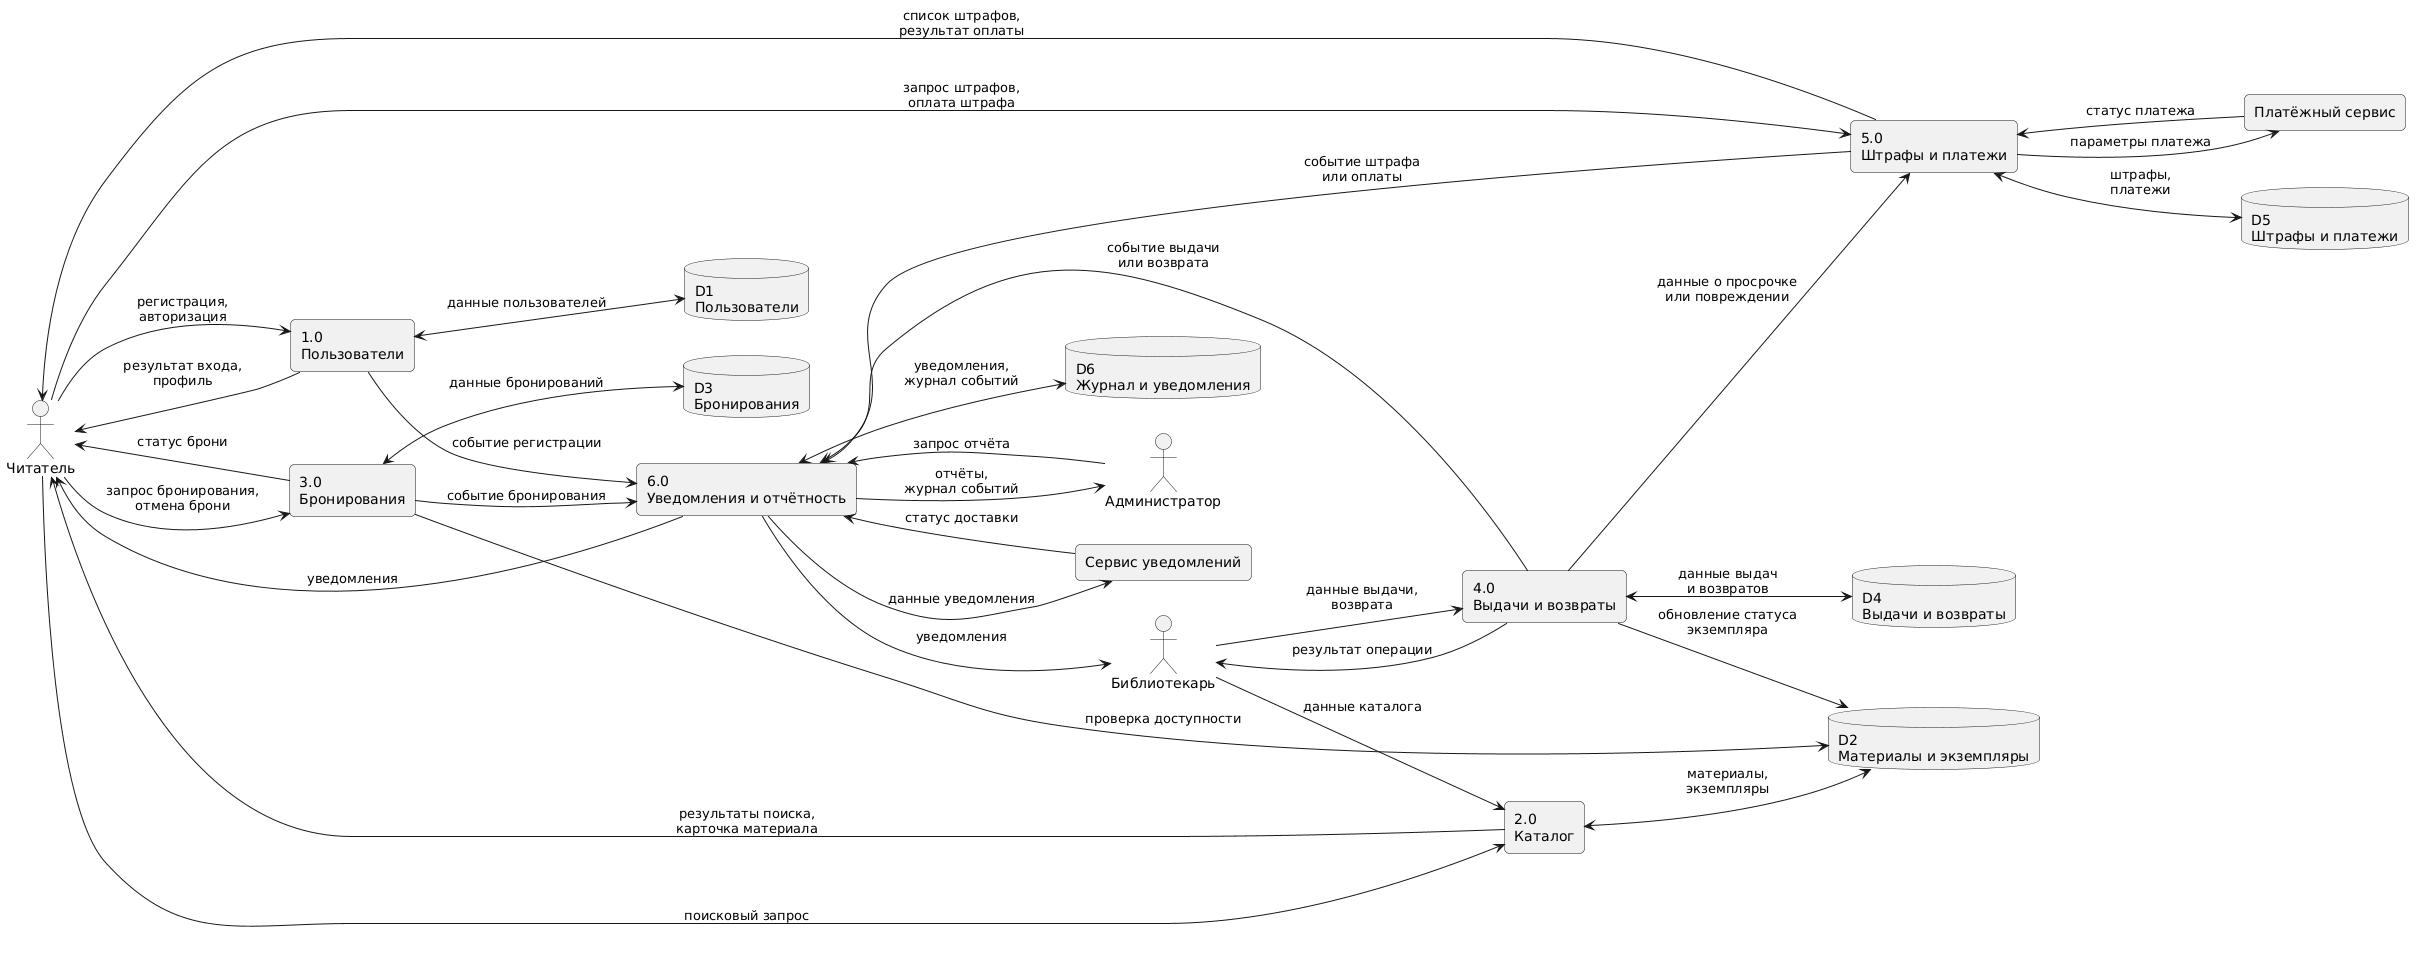
\includegraphics[width=1\textwidth]{DFD diagram.png}
		\caption{DFD-диаграмма верхнего уровня для Library Service}
		\label{fig:dfd-level-1}
	\end{figure}
	
	\subsection{Operating environment}
	
	Основное окружение работы системы включает следующие компоненты:
	
	\begin{description}
		\item[Backend-сервер]
		Серверная часть системы реализуется на Java с использованием Spring Framework.
		Backend-сервер обрабатывает пользовательские запросы, выполняет бизнес-логику,
		работает с базой данных, внешними сервисами и предоставляет REST API для
		клиентских приложений.
		
		\item[База данных]
		Для хранения данных системы используется PostgreSQL. В базе данных хранятся
		данные пользователей, материалов, экземпляров, бронирований, выдач, возвратов,
		штрафов, платежей, уведомлений и журнала событий.
		
		\item[Клиентские приложения]
		Система может использоваться через веб-приложение, мобильное приложение и
		десктопное приложение. Все клиентские приложения взаимодействуют с backend-сервером
		через HTTPS API и используют единые правила доступа к данным.
		
		\item[Веб-приложение]
		Веб-клиент предназначен для работы через современный браузер. Он может
		использоваться читателями, библиотекарями и администраторами.
		
		\item[Мобильное приложение]
		Мобильный клиент предназначен для использования читателями на мобильных
		устройствах. Он предоставляет доступ к поиску материалов, бронированиям,
		выдачам, уведомлениям и штрафам.
		
		\item[Десктопное приложение]
		Десктопный клиент может использоваться сотрудниками библиотеки для выполнения
		операционных задач: оформления выдачи и возврата, обработки бронирований и
		работы с каталогом.
		
		\item[Внешний платёжный сервис]
		Для оплаты штрафов система использует внешний платёжный сервис. Library Service
		передаёт параметры платежа и получает результат обработки операции.
		
		\item[Сервис уведомлений]
		Для отправки сообщений пользователям и сотрудникам библиотеки используется
		внешний почтовый или SMS-сервис. Система передаёт данные уведомления и получает
		статус доставки.
		
		\item[Средства мониторинга и журналирования]
		Для контроля состояния системы используются средства логирования, мониторинга
		и аудита. Они позволяют фиксировать ошибки, технические события и действия
		пользователей с повышенными правами.
	\end{description}
	
	Минимальное серверное окружение для развёртывания системы включает:
	
	\begin{itemize}
		\item операционную систему Linux, поддерживающую запуск JVM;
		\item установленную Java Runtime Environment (JRE) для запуска backend-приложения;
		\item сервер базы данных PostgreSQL;
		\item доступ к внешнему платёжному сервису;
		\item доступ к сервису отправки e-mail или SMS-уведомлений;
		\item сетевое соединение между клиентскими приложениями, backend-сервером и базой данных;
		\item поддержку HTTPS для защищённого обмена данными.
	\end{itemize}
	
	
	
\end{document}